% The mathematics of cooperation and attribution.

% insert an image right here
\begin{figure}[h]
    \centering
    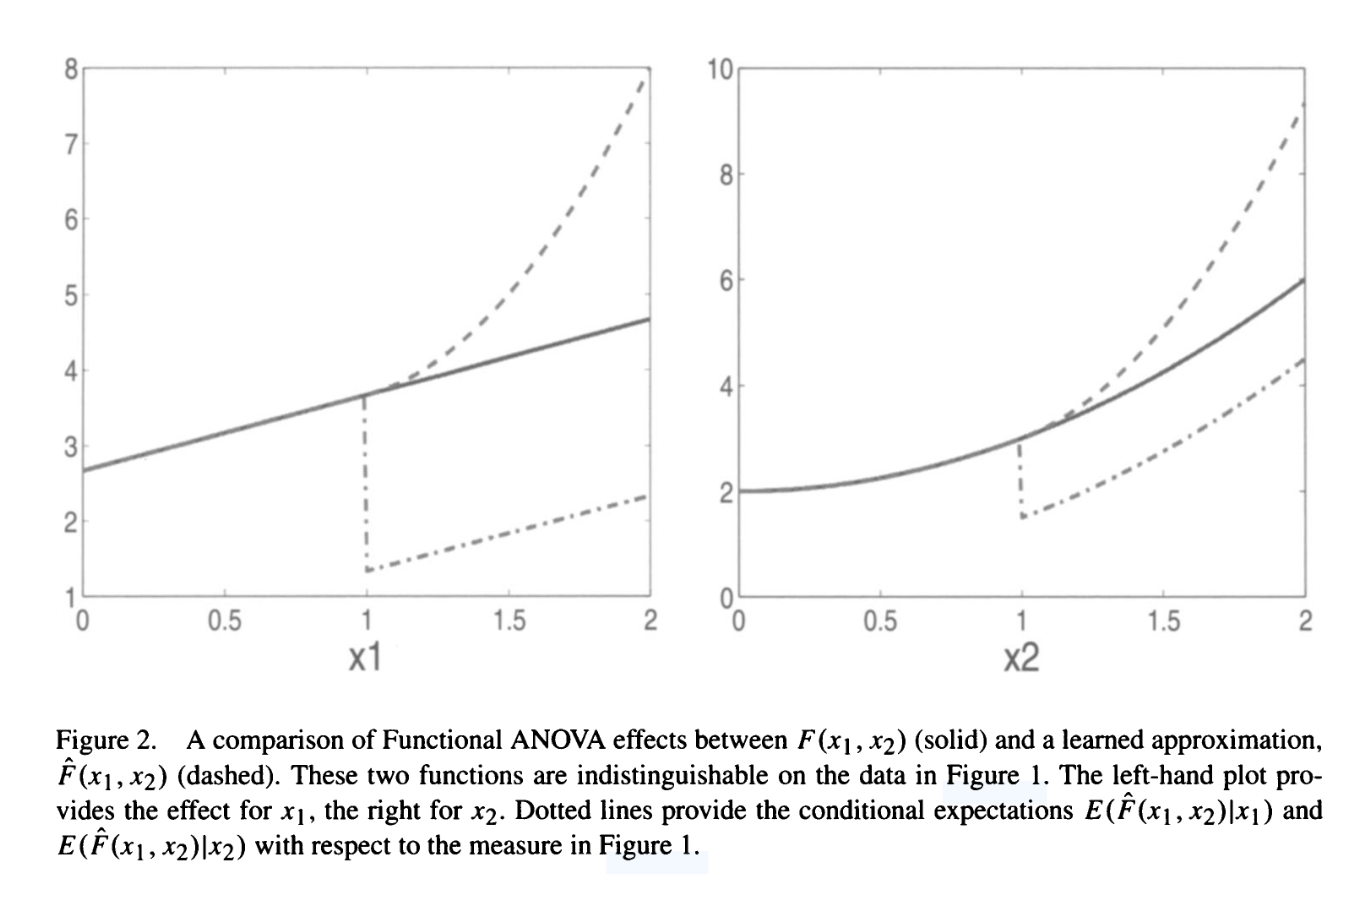
\includegraphics[width=0.8\textwidth]{images/hooker_2007_figure2.png}
    \label{fig:hooker_graph}
\end{figure}

\subsection*{Questions}
\begin{itemize}
    \item Can you reconstruct the function from only the fANOVA terms? I think it can be reconstructed only if variables are independent, have zero-mean, are orthogonal?
    \item Is it possible to perform fANOVA for non-square-integrable functions? I think in general yes but the variance decomposition doesn't work then or might have problems.
    \item fANOVA decomposition for discrete variables possible? Does it make sense even?
    % \item Denote original model with $y$ or $f$?
    \item Connection between the (conditional) expected value, (partial) integral, projections (section~\ref{general_definitions})?
    \item In the hierarchical orthogonality condition (4.2) formulated in \cite{hooker2007} for the gerneralized fAVNOA framework, shouldn't we explicitly exclude the case that $v = u$, because then, we would require that the inner product of the fANOVA component is zero wouldn't we (section~\ref{generalization})?
    \item I am a bit confused by Figure 2 in \cite{hooker2007} (see \autoref{fig:hooker_graph}), especially by the dotted line for conditional expectation. What should it tell us? I think what the dashed line (learned approximation) shows is that the model estimates a non-linear effect for x1, even though the true effect is linear. The reasons are the problematic data points in the top right region.
    % \item If the general fANOVA formulation is a true generalization then I should be able to take the general form and construct from it the simple form when I use certain constrains (such as independence, uniform distribution, etc.) right?
    \item Why is it a problem, when explainability methods also place large emphasis on regions of low probability mass when dependencies between variables exist - because in the end explainability is about explaining the model, not the data generating process; and after all it is how the model works in these regions. [But as the Hooker example illustrates, how the model works and what it estimates in these regions is wrong and then it's better to not report any model behaviour or come closer to the DGP than to give wrong estimations?]
    \item 
    \item Use of AI tools?
    \item Do we need to restrict ourselves to the unit hypercube? Or does fANOVA decomposition work in general, but maybe with some constraints? Originally it was constructed for models on the unit hypercube $[0,1]$, but other papers also use models from $R^d$ \textit{Generally no restriction, so next step could be to generalize, to $\mathbb{R}^n$, other measures, dependent variables}
    \item Still unclear: Are the terms fully orthogonal or hierarchically? See subsection on Orthogonality of the fANOVA terms (especially the example) I think in the original fANOVA decomposition the terms are orthogonal but in the generalized fANOVA \citep{hooker2007} they are hierarchically orthogonal. \textit{fully orthogonal when independence assumption, probably partially when no independence}
    \item $x_1, \dots, x_k$ are simply the standardized features, right? \textit{Yes}
    \item {\color{orange}My current understanding: we need independence of $x_1, \dots x_k$ so that fANOVA decomposition is unique (and orthogonality holds). We need zero-mean constraint for the orthogonality of the components. We need orthogonality for the variance decomposition.}\textit{zero-mean $\rightarrow$ orthogonality $\rightarrow$ uniqueness; Lemma 1 im Hooker 2007 ist verallgemeinerg ds zero-mean constraint}
    \item Next step might be to investigate the (mathematical) parallels of fANOVA decomposition and other IML methods (PDP, ALE, SHAP), e.g. there is definitely a strong relationship between Partial dependence (PD) and fANOVA terms, and PD is itself again related to other IML methods; Also look how are other IML models studied and study fANOVA in a similar way (e.g. other IML methods are defined, checked for certain properties, examined under different conditions (dependent features, independent features) etc.) (see dissertation by Christoph Molnar for this); Also I would be very interested in investigating the game theory paper further \citep{fumagalli2025} but still a bit unsure if it is too complex.
    \item Why does a fANOVA decomposition of a simple GAM not lead to the ``true'' coefficients? \href{https://christophm.github.io/interpretable-ml-book/decomposition.html}{https://christophm.github.io/interpretable-ml-book/decomposition.html} talks about this a bit in the subchapter ``Statistical regression models'' \textit{It should actually lead to the GAM; at least under all the constraint like zero-mean constraint and orthogonality}
    \item 
    \item In \cite{hooker2004} they work with $F(x)$ and $f(x)$, but in \cite{sobol2001} they only work with $f(x)$. I think this is only notation? \textit{Only notation.}
    \item Does orthogonality in fANOVA context mean that all terms are orthogonal to each other? Or that a term is orthogonal to all lower-order terms (\ldq Hierarchical orthogonality \rdq)? \textit{The terms are hierarchically orthogonal, so each term is orthogonal to all lower-order terms, but not to the same-order terms! So $f_1$ is not necessarily orthogonal to $f_2$ but it is orthogonal to $f_{12}$, $f_{0}$.} 
    \item Do the projections here serve as approximations? (linalg skript 2024 5.7.4 Projektionen als beste Annäherung) \textit{Yes, they can be interpreted as sort of approximation.}
    \item Which sub-space are we exactly projecting onto? Are the projections orthogonal by construction (orthogonal projections) or only when the zero-mean constraint is set? \textit{The subspace we project onto depends on the component. For $f_0$ we project onto the subspace of constant functions, for $f_1$ we project onto the subspace of all functions that involve $x_1$ and have an expected value of 0 (zero-mean constraint to ensure orthogonality). It depends on the formulation of the fANOVA decomposition if you need to explicitly set the zero-mean constraint for orthogonality or if it is met by construction.}
    \item How \ldq far\rdq should I go back, formally introduce $L^2$ space, etc. or assume that the reader is familiar with it? \textit{Yes, space, the inner product on this space should be formally introduced.}
    % \item zero mean condition vs. zero-sum condition: according to GPT zero mean condition is related to orthogonality and zero-sum to the additivity
\end{itemize}

\section*{fANOVA Brainstorming Questions}

\subsection*{What happens if...?}
\begin{itemize}
    \item What happens if the function \( f \) is linear in all its variables? What do the fANOVA terms look like in that case?
    \item What happens if some variables are independent? Do any Sobol’ terms vanish automatically?
    \item What happens if you permute the inputs? Do the Sobol’ indices change?
    \item What happens if two variables are strongly collinear? How does that affect the interpretability of fANOVA?
\end{itemize}

\subsection*{Why is...?}
\begin{itemize}
    \item Why is orthogonality (zero mean and mutual independence of components) important in fANOVA?
    \item Why is the constant term \( f_0 \) equal to the expected value of \( f \)?
    \item Why is fANOVA usually associated with variance-based methods like Sobol indices?
    \item Why is it necessary to subtract lower-order terms when computing higher-order ones?
    \item Why is the decomposition hierarchical?
\end{itemize}

\subsection*{Is it possible to...?}
\begin{itemize}
    \item Is it possible to compute fANOVA in closed form for certain functions (e.g., polynomials)?
    \item Is it possible to use fANOVA in models where inputs are dependent?
    \item Is it possible to extend fANOVA to time-series models or dynamic systems?
    \item Is it possible to use fANOVA ideas in neural networks? How would you interpret interactions then?
\end{itemize}

\subsection*{What does this remind you of? (Analogies and Parallels)}
\begin{itemize}
    \item fANOVA reminds me of \emph{Fourier decomposition}: projecting a function onto orthogonal basis functions.
    \item It feels similar to \emph{PCA}, but in the input space instead of the output space.
    \item fANOVA terms are like \emph{partial derivatives} in symbolic differentiation — quantifying localized influence.
    \item It’s analogous to \emph{ANOVA in statistics}, but instead of experimental groups, you decompose function behavior.
    \item In machine learning, it reminds me of \emph{feature importance} in random forests or \emph{Shapley values}.
    \item fANOVA’s additive structure is similar to \emph{GAMs (Generalized Additive Models)}.
\end{itemize}

\subsection*{How does fANOVA compare to...?}
\begin{itemize}
    \item How does fANOVA compare to Shapley values? (Shapley is axiomatic, fANOVA is Hilbert space projection-based.)
    \item How does fANOVA compare to LIME/SHAP in interpretability?
    \item How does fANOVA compare to gradient-based sensitivity methods?
    \item How does fANOVA compare to partial dependence plots?
    \item How does fANOVA compare to mutual information as a dependence measure?
\end{itemize}
